\documentclass[19pt,landscaoe]{article}
\usepackage[landscape]{geometry}
\geometry{a5paper,scale=0.8}
\usepackage{listings}
%\geometry{left=1.5cm,right=1.5cm,top=1.5cm,bottom=0.5cm}
\usepackage{color}
% \usepackage{ulem} % for strikethrough
\usepackage{amsfonts}
\usepackage{bm}
\usepackage{graphicx} 
\usepackage{amsfonts,amsmath,latexsym,amssymb,mathrsfs,amsthm,mathtools}
% \usepackage[british]{babel}
%\usepackage[T1]{fontenc}
%\usepackage{mathptmx}
% \usepackage{times}
\usepackage{datetime2}
\usepackage{filemod}
% \usepackage{fontspec}    %change font 
% \setmainfont{Times New Roman}%fontspec下这个命令设置全局默认字体
\newtheorem{thm}{Theorem}%[section]
\newtheorem{prop}[thm]{Proposition}
\newtheorem{defi}[thm]{Definition}
\newtheorem{lma}[thm]{Lemma}
\newtheorem{cor}[thm]{Corollary}
\newtheorem{exam}[thm]{Example}
\newtheorem{countexam}[thm]{Counterexample}
\newtheorem{rem}[thm]{Remark}
\newtheorem{con}[thm]{Conjecture}
%\bracketfactory{floor}{\lfloor}{\rfloor}
\usepackage{enumerate}
\usepackage{color}
%\usetheme{Copenhagen}
\usepackage[english]{babel}
\usepackage[utf8x]{inputenc}
\newcommand{\law}{\mathscr{L}}
\newcommand{\HH}{\mathscr{H}}
\newcommand{\D}{\mathbb{D}}
\newcommand{\IP}{\mathbb{P}} 
\newcommand{\bone}{{\bf 1}}
\DeclareMathOperator{\E}{\mathbb{E}}
\DeclareMathOperator*{\esssup}{ess\,sup}
\newcommand{\IE}{\E}
\newcommand{\mean}{\E}
\newcommand{\R}{\mathbb{R}}
\newcommand{\N}{\mathbb{N}}
\newcommand{\non}{\nonumber}
\newcommand{\Z}{\mathbb{Z}}
\newcommand{\C}{\mathbb{C}}
%\newcommand{\C}{{\mathds{C}}}
\newcommand{\ci}{{\cal I}}
\newcommand{\cf}{{\cal F}}
\newcommand{\LL}{\textbf{L}}
\DeclareMathOperator{\Var}{\mathrm{Var}}
\DeclareMathOperator{\var}{\mathrm{Var}}
\DeclareMathOperator{\cov}{\mathrm{Cov}}
\DeclareMathOperator{\corr}{\mathrm{Corr}}
\DeclareMathOperator{\bs}{\mathrm{Bias}}
\DeclareMathOperator{\bigo}{\mathrm{O}}
\newcommand{\K}{\textbf{Ker}}
\newcommand{\Id}{\textbf{Id}}
\newcommand{\Pn}{{\rm Pn}}
\newcommand{\dtv}{{d_{\rm TV}}}
\newcommand{\dk}{{d_{\rm K}}}
\newcommand{\dw}{{d_{\rm W}}}
\def\tg{{\tilde g}}
\def\a{{\alpha}}
\def\cn{{\mathcal{N}}}
\def\equald{\stackrel{\mbox{\scriptsize{{\rm d}}}}{=}}
\def\ER{Erd\H{o}s-R\'enyi}
\usepackage{color} 
\definecolor{lightblue}{rgb}{0,0.2,0.5}
\usepackage[colorlinks=true, urlcolor=lightblue,linkcolor=lightblue, citecolor=lightblue]{hyperref}

%%%%%%%%%%%%%%%%%%%%%%%%%%%%%%%%%%

%%% Define bracket commands
\def\given{\mskip 0.5mu plus 0.25mu\vert\mskip 0.5mu plus 0.15mu}
\newcounter{@bracketlevel}
\def\@bracketfactory#1#2#3#4#5#6{
\expandafter\def\csname#1\endcsname##1{%
\addtocounter{@bracketlevel}{1}%
\global\expandafter\let\csname @middummy\alph{@bracketlevel}\endcsname\given%
\global\def\given{\mskip#5\csname#4\endcsname\vert\mskip#6}\csname#4l\endcsname#2##1\csname#4r\endcsname#3%
\global\expandafter\let\expandafter\given\csname @middummy\alph{@bracketlevel}\endcsname
\addtocounter{@bracketlevel}{-1}}%
}
\def\bracketfactory#1#2#3{%
\@bracketfactory{#1}{#2}{#3}{relax}{0.5mu plus 0.25mu}{0.5mu plus 0.15mu}
\@bracketfactory{b#1}{#2}{#3}{big}{1mu plus 0.25mu minus 0.25mu}{0.6mu plus 0.15mu minus 0.15mu}
\@bracketfactory{bb#1}{#2}{#3}{Big}{2.4mu plus 0.8mu minus 0.8mu}{1.8mu plus 0.6mu minus 0.6mu}
\@bracketfactory{bbb#1}{#2}{#3}{bigg}{3.2mu plus 1mu minus 1mu}{2.4mu plus 0.75mu minus 0.75mu}
\@bracketfactory{bbbb#1}{#2}{#3}{Bigg}{4mu plus 1mu minus 1mu}{3mu plus 0.75mu minus 0.75mu}
}


% \title{Nonparametric Regression}
% \author{Qingwei Liu}
% \institute{National University of Singapore}
% \date{\today}

\begin{document}
% \maketitle
%

% \begin{titlepage}
% \begin{center}
%     \vfill
% \textbf{\huge ST5207 Nonparametric Regression\\
% Semester 1, AY2024/25}\\[4cm]
% \begin{minipage}{0.4\textwidth}
% \begin{center} \large
% Lecturer:~Qingwei Liu\\
% % Email:liu\_qw@nus.edu.sg\\
% \vskip 6pt
% Department of Statistics and Data Science\\
% \vskip 6pt
% National University of Singapore
% \end{center}
% \end{minipage}%\\[1cm]
% \vfill
% % \includegraphics[width=0.1\textwidth]{./logo}\\[0.5cm]
% \vfill
% \end{center}

% \end{titlepage}
%

\newpage
\centering{\LARGE\textbf{Lecture~2:~Histogram Method} for nonparametric density estimation\footnote{Last modified in \filemodprintdate{Lecture2}.}}
\vskip25pt
\begin{minipage}{.9\textwidth}
    \Large
\begin{itemize}
\item The Empirical  Distribution Function Estimator
\item The naive Estimator 
\item The Histogram Estimator  
\item Asymptotics of the Histogram Estimator 
\item Bin number selection

\end{itemize}
\end{minipage}
\newpage
{\Large\centerline{\textbf{Problem}}}
\vskip25pt
\begin{minipage}{.9\textwidth}
    \Large
Let $X$ be a continuous random variable with cumulative distribution function (c.d.f.) $F$ and p.d.f. $f$.
(Both c.d.f. and p.d.f. characterize the distribution.)
In practice, the distribution of $X$ is in general unknown. All you have are $n$ observations $X_1,\dots,X_n$ of $X$, in other words, i.i.d. samples with size $n$. 
\vskip 10pt
{\bf Problem:}~~~How do you estimate $f(\cdot)$ using those samples? 
\vskip 5pt
Note, we don't assume that $f(\cdot)$ has some known functional form except for some unknown parameter(s) that need to be estimated. (That is exactly the parametric approach.)
\vskip 5pt
We will focus on nonparametric ways of estimating $f(\cdot)$ instead. 
% In one hand, we know from second-year probability theory,
% \begin{equation}
%     f(x)=\frac{\mathrm{d}F(x)}{\mathrm{d}x}=\lim_{h\to0}\frac{F(x+h)-F(x-h)}{2h}
% \end{equation}
\end{minipage}

\newpage
{\LARGE\centerline{\textbf{Empirical distribution function}}}
\vskip25pt
\begin{minipage}{.9\textwidth}
    \Large The simplest function to estimate nonparametrically is the c.d.f. $F$ of random variable $X$. 
From elementary probability theory, the {\it empirical distribution function} (EDF), defined as, for any $x\in\R$, 
\begin{equation}
    F_n(x):=\frac1n\sum_{i=1}^n\bone_{\{X_i\le x\}},
\end{equation}
is a straightforward estimator for $F(x)$. 
\vskip 5pt
For any fixed $x\in\R$, $\bone_{\{X_i\le x\}}$ is a Bernoulli RV with mean $F(x)$. As a consequence, $F_n(x)$ is a RV with mean 
\begin{equation*}
    \E[F_n(x)]=\E\left(\bone_{\{X_1\le x\}}\right)=\IP(X_1\le x)=F(x),
\end{equation*}
and variance 
\begin{equation*}
    \Var(F_n(x))=\frac1{n^2}\cdot n\Var(\bone_{\{X_i\le x\}})=\frac1nF(x)\left(1-F(x)\right).
\end{equation*}
\end{minipage}

\newpage
{\LARGE\centerline{\textbf{A native estimator}}}
\vskip25pt
\begin{minipage}{.9\textwidth}
    \Large 
    Therefore, $F_n(x)$ is a {\it consistent unbiased} estimator of $F(x)$. 

    \vskip 5pt
    In particular, EDF allocates equal weight $n^{-1}$ on each datum point.
    \vskip 5pt
    On the other hand, inspired by EDF, it is easy to write 
    \begin{eqnarray*}
        f(x)&=&\lim_{h\to0}\frac{F(x+h)-F(x-h)}{2h}\\
        &=&\lim_{h\to0}\frac{\E\left[\bone_{\{x-h<X_i\le x+h\}}\right]}{2h}\\
        &=&\lim_{h\to0}\E\left[\frac{\sum_{i=1}^n\bone_{\{x-h<X_i\le x+h\}}}{2nh}\right].
    \end{eqnarray*}
    Hence, we obtain a {\it native estimator} for the density function $f(\cdot)$, 
\begin{equation}\label{def-nat}
    \hat{f}_n(x):=\frac1{2nh}\sum_{i=1}^n\bone_{\{x-h<X_i\le x+h\}},
\end{equation}
    for some $h>0$ small. 
\end{minipage}

\newpage
{\LARGE\centerline{\textbf{Histogram Estimator}}}
\vskip25pt
\begin{minipage}{.9\textwidth}
    \Large
The histogram is the oldest and the most commonly used nonparametric density estimator. The construction of histogram is almost the same as the naive estimator.  
\begin{itemize}
   \item Choose an origin $x_0$, and {\it binwidth} $h>0$;
   \item Denote the {\it bins} of the histogram as 
   $$B_j:=[x_0+jh,x_0+(j+1)h),~~~j\in\Z.$$
\end{itemize}
The histogram is given by 
\begin{equation}\label{def-hist}
    \widehat{f}_h(x):=\frac1{nh}\sum_{i=1}^n\sum_{j}\bone_{\{X_i\in B_j\}}\bone_{\{x\in B_j\}}.
\end{equation}
\end{minipage}
% \newpage
% {\LARGE{\textbf{Parametric Modeling}}}
% \vskip25pt
% {\Large\bf{Examples}}
   
% \begin{figure}[h]
% 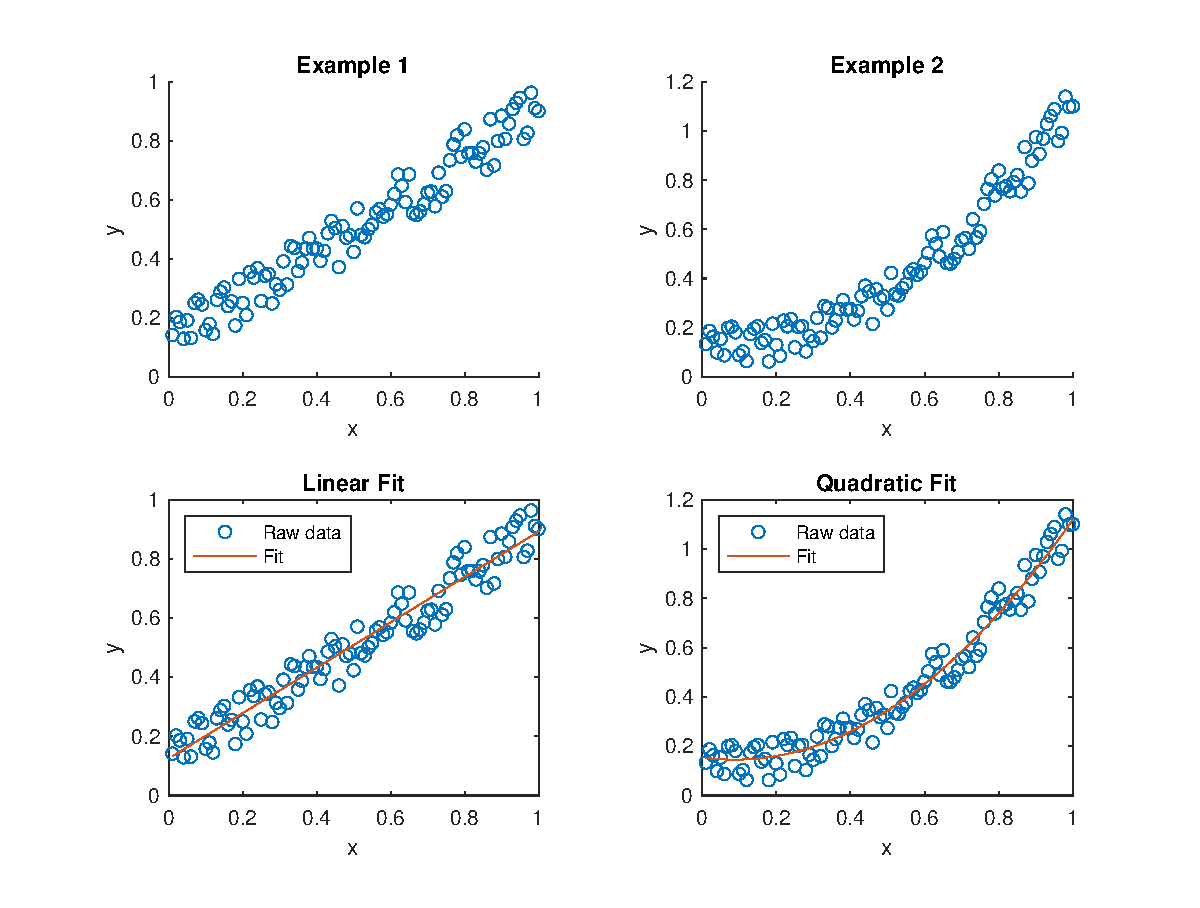
\includegraphics[width=0.8\textwidth,height=0.5\textwidth]{figure1.eps}
%     \label{figure1} 
% \end{figure}

\newpage
{\LARGE{\textbf{Comparsion of Naive and Histogram}}}
\vskip25pt
\begin{minipage}{.9\textwidth}
    \Large 
    We may assume  $x_0=0,$ and $x\in B_j=[jh,(j+1)h]$, without loss of generality (w.l.o.g.), and rewrite \eqref{def-hist} as  
    \begin{equation}\label{refine-hist}
        \widehat{f}_h(x):=\frac1{nh}\sum_{i=1}^n\bone_{\{X_i\in B_j\}}.
    \end{equation}
    Comparing \eqref{def-nat} with \eqref{refine-hist}, we can see 
    % \Large
\begin{itemize}
\item The naive estimator is defined in a pointwise manner. For each $x$ fixed, take a neighborhood of $x$ with fixed radius $h$.
\item Bins appeared in \eqref{def-hist} is independent of $x$, and purely determined by the selection of origin $x_0$ and binwidth $h$.
\end{itemize}
\end{minipage}

% \newpage
% {\LARGE{\textbf{Parametric Modeling}}}
% \vskip25pt
% {\Large\bf{Scatter plot of raw data}}

% \begin{figure}[h]
% \centering
% 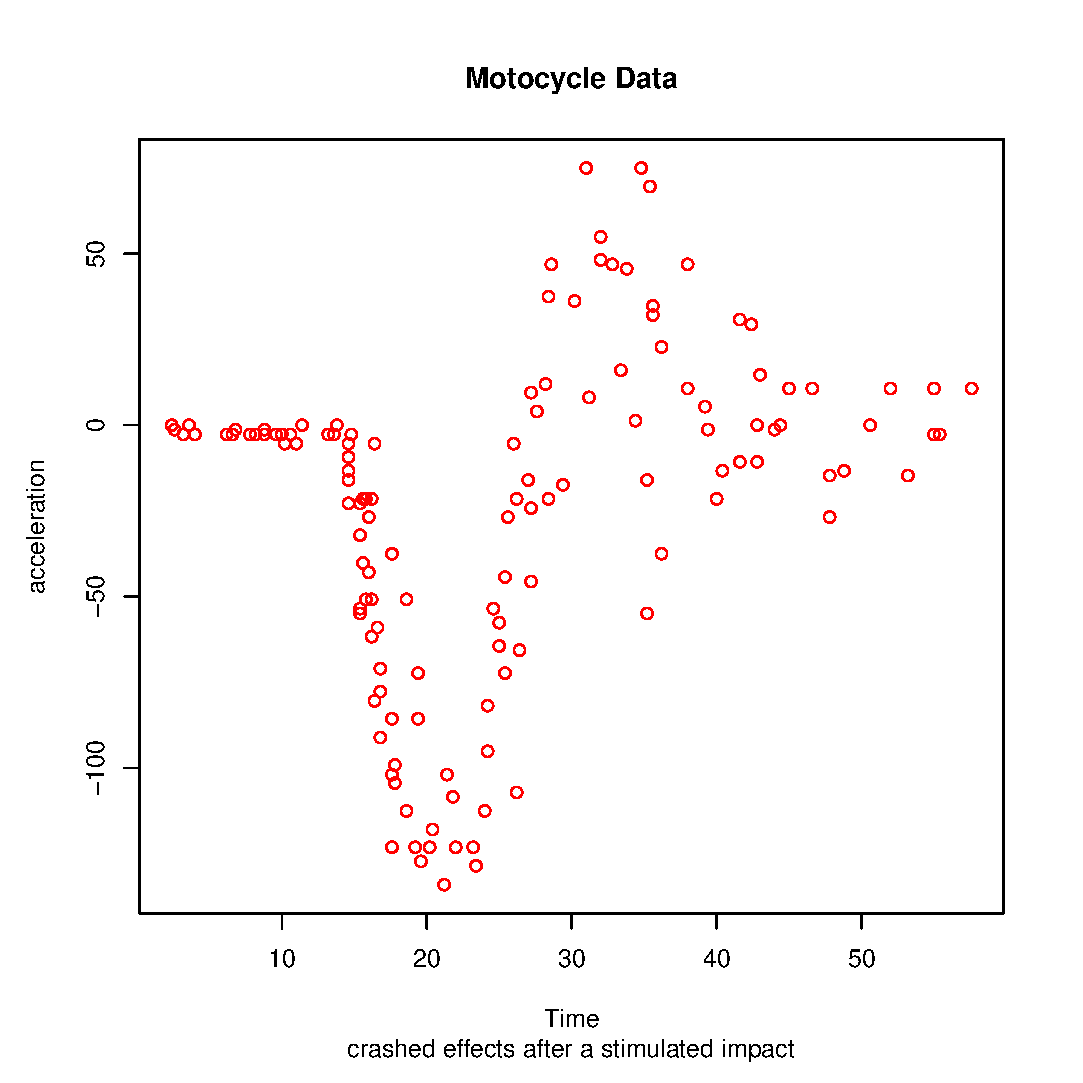
\includegraphics[width=0.75\textwidth,height=0.52\textwidth]{MotocycleData.eps}
%     \label{figure2} 
% \end{figure}

% \newpage
% {\LARGE{\textbf{Parametric Modeling}}}
% \vskip25pt
% {\Large\bf{Polynomial Fit}}

% \begin{figure}[h]
% \centering
%       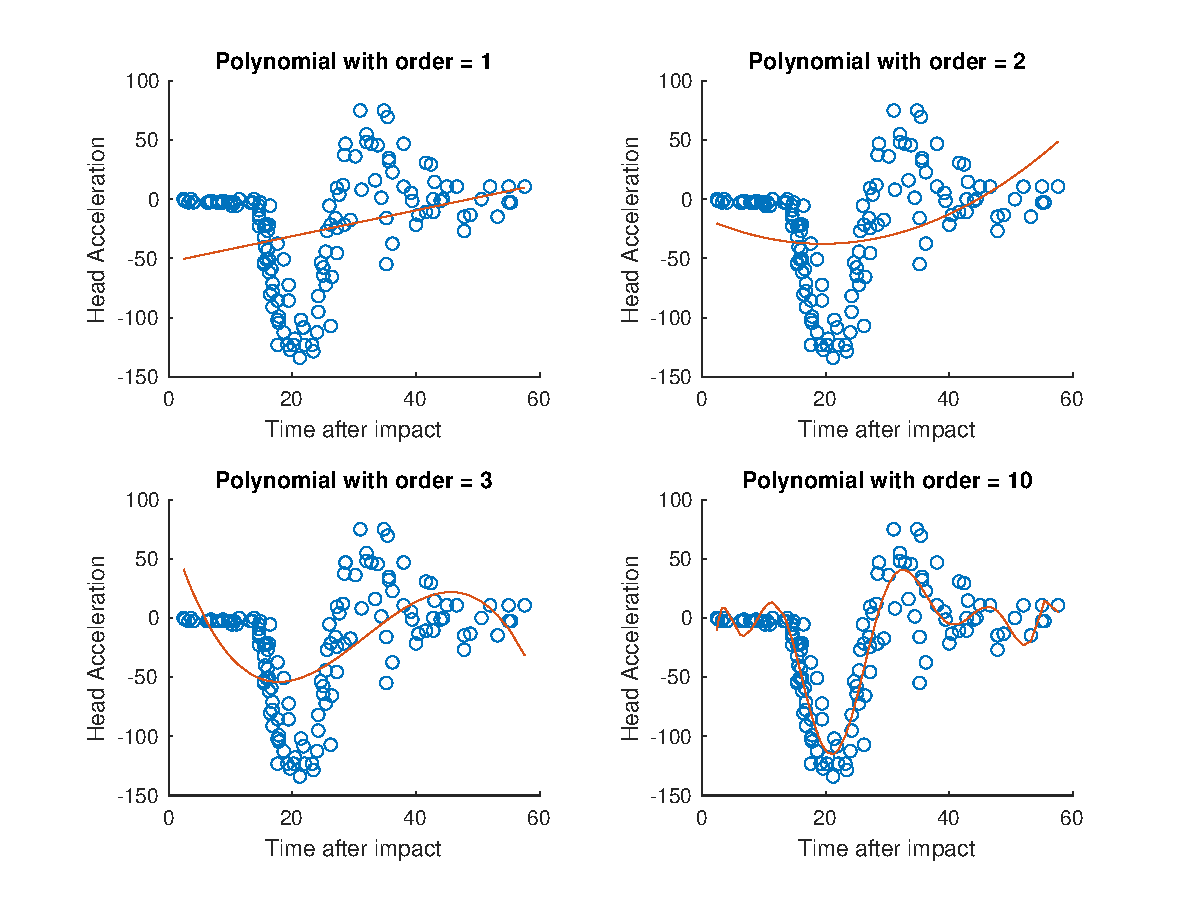
\includegraphics[width=0.75\textwidth,height=0.52\textwidth]{polyfitting.eps}
%     \label{figure3} 
% \end{figure}

\newpage
{\LARGE\centerline{\textbf{Statistical Properties}}}
\vskip25pt
\begin{minipage}{.9\textwidth}
    \Large
    \begin{itemize}
        \item Bias: 
        \begin{eqnarray}
            \bs\left\{\widehat{f}_h(x)\right\}&=&\E\left[\widehat{f}_h(x)\right]-f(x)\nonumber\\
            &=&h^{-1}\IP\left(X_1\in B_j\right)-f(x)\nonumber\\
            &=&\frac1h\int_{B_j}f(u)\mathrm{d}u-f(x)\nonumber\\
            &=&f(u^*)-f(x),\label{bs-mvt}
        \end{eqnarray}
        where the last equity is due to the Mean Value Theorem for some $u^*\in B_j$. 
    \end{itemize}
Intuitively, we may think the bias will vanish as the binwidth $h\to0$. Nope. We need certain {\bf stronger} condition on the density function $f(\cdot)$ to ensure this. So far, we only assume the existence of $f(\cdot)$.
\end{minipage}

\newpage
{\LARGE\centerline{\textbf{Statistical Properties (cont.)}}}
\vskip25pt
\begin{minipage}{.9\textwidth}
    \Large
    \begin{itemize}
        \item Variance:
        \begin{eqnarray}
            \var\left(\widehat{f}_h(x)\right)&=&\frac1{(nh)^2}\var\left(\sum_{i=1}^n\bone_{\{X_i\in B_j\}}\right)\nonumber\\
            &=&(nh^2)^{-1}\var\left(\bone_{\{X_1\in B_j\}}\right)\nonumber\\
            &=&(nh^2)^{-1}p_x(1-p_x)\\
            &=&(nh)^{-1}f(u^*)(1-p_x)\label{var-bound1}
        \end{eqnarray}
        where $p_x:=\int_{B_j}f(u)\mathrm{d}u$.
    \end{itemize}
From the last equality, it is not difficult to see that for $n$ fixed 
$$\var\left(\widehat{f}_h(x)\right)\to\infty,~~~~\mathrm{as}~~~h\to0.$$ 
\end{minipage}


\newpage
{\LARGE\centerline{\textbf{Continuity condition and MSE}}}
\vskip25pt
\begin{minipage}{.9\textwidth}
    \Large
        For a function $g:\R\to\R$, suppose that for any $x,y\in\R$, it holds 
        \begin{equation}
            |g(x)-g(y)|\le K|x-y|^\alpha,
        \end{equation}
        for some $\alpha>0$. 
        For $\alpha=1$, such functions are called {\it Lipschitz functions}. For $0<\alpha<1$, they are said to satisfy a {\it H\"older condition} of order $\alpha$, c.f.\cite[Page~56]{Dudley02}. 
\vskip 5pt
        For a function $g$ defined on a finite interval $[a,b]$ with $a<b$, 
        $$\mathrm{Lipschitz~continous}\Rightarrow \mathrm{H\ddot{o}lder~continuous}\Rightarrow \mathrm{uniformly~continuous}.$$
Mean Square Error (MSE) of $\widehat{f}_h(x)$, defined by 
\begin{eqnarray}
    {\rm MSE}\left\{\widehat{f}_h(x)\right\}:=\E\left[\left|\widehat{f}_h(x)-f(x)\right|^2\right],
\end{eqnarray}
is a widely used performance measure of an estimator. 
\end{minipage}

\newpage
{\LARGE\centerline{\textbf{Main Theorem}}}
\vskip25pt
\begin{minipage}{.9\textwidth}
    \large
\begin{thm}\label{thm1-L2}
    Suppose the density function $f$ is Lipschitz continuous on the interval $B_j$. When $n^{-1}\ll h\ll1$, the histogram $\widehat{f}_h(x)$ converges to $f(x)$, in the mean square sense,  i.e. 
    \begin{equation}
        {\rm MSE}\left\{\widehat{f}_h(x)\right\}\to0,
    \end{equation}
    as $n\to\infty$.
\end{thm}
\begin{proof}
    Since $f$ is Lipschitz continuous on $B_j$, from \eqref{bs-mvt}, we have
    \begin{equation}\label{bs-bound}
        \left|\bs\left\{\widehat{f}_h(x)\right\}\right|=\left|f(u^*)-f(x)\right|\le K|u^*-x|\le Kh.
    \end{equation}
    Furthermore, from \eqref{var-bound1}, we have 
    \begin{equation}\label{var-bound2}
        \var\left(\widehat{f}_h(x)\right)\le C(nh)^{-1}
    \end{equation} for some constant $C$, 
    as $f$ is bounded on $B_j$, implied by the Lipschitz continuity. Combining \eqref{bs-bound} with \eqref{var-bound2}, we have
    \begin{equation} \label{bound-mse1}
        {\rm MSE}\left\{\widehat{f}_h(x)\right\} =\left(\bs\left\{\widehat{f}_h(x)\right\}\right)^2+\var\left(\widehat{f}_h(x)\right)\le K^2h^2+C(nh)^{-1}\to0.
    \end{equation}
\end{proof}
{\small An easy trick: $E(X-a)^2=\E(X-\E(X)+\E(X)-a)^2=\Var(X)+(\E(X)-a)^2$.}
\end{minipage}

\newpage
{\LARGE\centerline{\textbf{Selection of binwidth}}}
\vskip25pt
\begin{minipage}{.9\textwidth}
    \Large The binwidth $h$ is referred to be a {\it smoothing parameter} in the literature on smoothing. 

    The inequality in \eqref{bound-mse1} summarizes the trade-off between bias and variance is determined by the choice of smoothing parameter. 

    We can take the upper bound in \eqref{bound-mse1} as a function of $h$, and achieve its minimal point at $h_{\min}:=[C(2nK^2)^{-1}]^{1/3}$. 
    
    Plugging $h_{\min}$ in \eqref{bound-mse1}, we have
    $${\rm MSE}\left\{\widehat{f}_h(x)\right\}=O\left(n^{-2/3}\right).$$
    Note, if we assume $f$ satisfying H\"older condition of order $\alpha$, for some $0<\alpha<1$, instead of Lipschitz continuity in Theorem~\ref{thm1-L2}, we can obtain 
    $${\rm MSE}\left\{\widehat{f}_h(x)\right\}=O\left(n^{-\frac{2\alpha}{2\alpha+1}}\right).$$
\end{minipage}

\newpage
{\LARGE\centerline{\textbf{Bin number selection}}}
\vskip25pt
\begin{minipage}{.9\textwidth}
    \Large 
\begin{itemize}
    \item Sturges' rule, c.f. \cite{sturges26};
    \item Doane's formula, c.f. \cite{doane76};
    \item Scott's rule, c.f. \cite{scott79};
    \item Freedman-Diaconis rule, c.f. \cite{FreedmanDiaconis81}. 
\end{itemize}
\end{minipage}

\newpage
{\LARGE{\textbf{Sturges' rule}}}
\vskip25pt
\begin{minipage}{.9\textwidth}
    \Large 
{\it Sturges' rule} is a method of selecting the number of bins for a histogram, being widely employed in statistical and data analysis software, including Python and R. 

Originating from the idea that using (symmetric) binomial distribution to approximate discretized normal distribution, \cite{sturges26} considers an idealized histogram with $k$ bins, where the $i$-th bin count is binomial coefficient ${k-1 \choose i}$, for $i=0,1,\dots,k-1$. As $k$ increase, this ideal histogram approaches the shape of a normal density. 

The total sample size is 
$$n=\sum_{i=0}^{k-1}{k-1 \choose i}=(1+1)^{k-1}=2^{k-1},$$
by the binomial formula. Sturges' rule for number of bins follows immediately:
\begin{equation}\label{sturges-rule}
    k=1+\log_2n.
\end{equation}
\end{minipage}

\newpage
{\LARGE{\textbf{Doane's rule}}}
\vskip15pt
\begin{minipage}{.9\textwidth}
    \Large 
If the data are not normal distributed, but are skewed, additional bins may be necessary. \cite{doane76} proposes increases the number of bins in \eqref{sturges-rule} by 
\begin{equation}\label{doane-rule}    k=\log_2(1+\hat{\gamma}_3\sqrt{n/6}),
\end{equation}
where 
$$\hat{\gamma}_3=\frac{n^{-1}\sum_{i=1}^n(x_i-\bar{x})^3}{(n^{-1}\sum_{i=1}^n(x_i-\bar{x})^2)^{3/2}}$$
is an estimate of the standardized skewness coefficient. 
\end{minipage}

\newpage
{\LARGE{\textbf{Mean Integrated Squared Error}}}
\vskip15pt
\begin{minipage}{.9\textwidth}
    \Large 
Instead of focusing on the accuracy of $\widehat{f}_h(x)$ as an estimator of $f$ at one single point, people are more likely to be interested in a global measure of accuracy. The most widely used global measure of estimation accuracy is the {\it mean integrated squared error} (MISE), 
\begin{eqnarray}
    {\rm MISE}\{\widehat{f}_h\}&:=&\E\left[\int_{\R}\left(\widehat{f}_h(x)-f(x)\right)^2\mathrm{d}x\right]\\
&=&\int_{\R}\E\left[\left(\widehat{f}_h(x)-f(x)\right)^2\right]\mathrm{d}x\nonumber\\
&=&\int_{\R}{\rm MSE}\{\widehat{f}_h(x)\}\mathrm{d}x.
\end{eqnarray}

\end{minipage}

\newpage
{\LARGE{\textbf{Mean Integrated Squared Error (cont.)}}}
\vskip15pt
\begin{minipage}{.9\textwidth}
    \Large 
    With stronger assumptions on the derivative $f'$, the asymptotic MISE is\footnote{See \cite[Section~3.2]{scott15} for more detailed analysis.}
    $${\rm AMISE}(h)=\frac1{nh}+\frac1{12}h^2\|f'\|_2^2.$$
    Hence, as we did for \eqref{bound-mse1}, minimizing at $h^*=\left[\frac6{n\|f'\|_2^2}\right]^{1/3}$, 
    \begin{equation}
    {\rm AMISE}(h^*)=(3\|f'\|_2/4)^{2/3}n^{-2/3}.
    \end{equation}
    Taking the density of normal distribution $\mathcal{N}(\mu,\sigma^2)$ as a reference, $\|f'\|_2^2=(4\sqrt{\pi}\sigma)^{-1}$
    \begin{equation}
        h^*=(24\sqrt{\pi})^{1/3}\sigma n^{-1/3}\approx 3.5\sigma n^{-1/3}.
        \end{equation}
        \begin{itemize}
            \item Scott's rule: $\hat{h}=3.5\hat{\sigma}n^{-1/3}$;
            \item Freedman-Diaconis's rule: $\hat{h}=2({\rm IQR})n^{-1/3},$ where ${\rm IQR}$ is the interquartile range. 
        \end{itemize}
\end{minipage}

\newpage
{\LARGE\centerline{\textbf{Summary}}}
\vskip25pt
\begin{minipage}{.9\textwidth}
    \Large 
    The optimal $O(n^{-2/3})$ for AMISE is unsatisfactorily slow, as \cite{boydsteele78} shows the best possible rate is $O(n^{-1})$ in the parametric approach. This deficiency can be regarded as the price for generality, i.e. removing parametric assumptions.  
\end{minipage}


\newpage
{\LARGE{\textbf{Histogram in R}}}
\vskip25pt

\begin{figure}[h]
\centering
      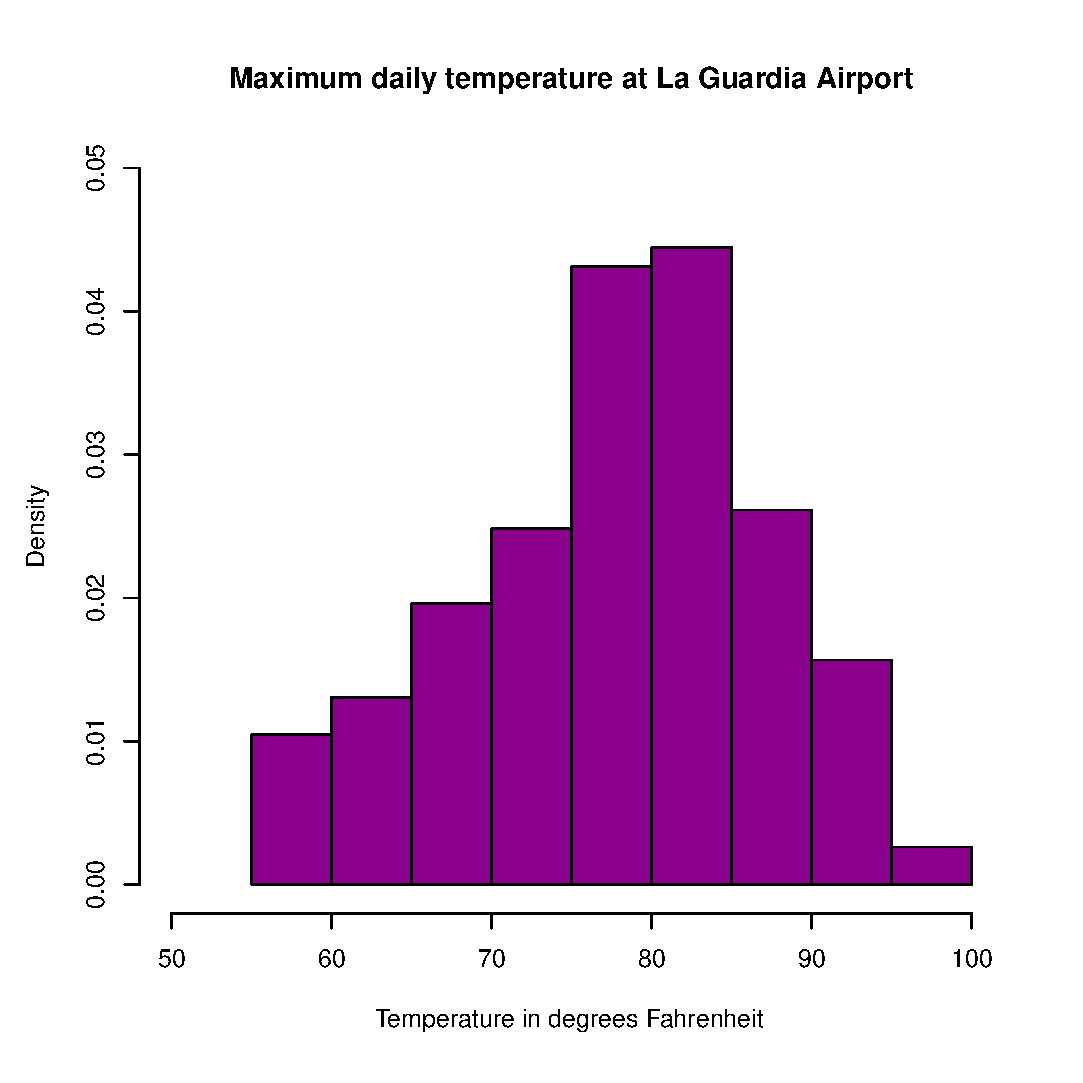
\includegraphics[width=0.75\textwidth,height=0.52\textwidth]{temperature.eps}
    \label{figure5} 
\end{figure}
(Data source: built-in dataset airquality which has "Daily air quality measurements in New York, May to September 1973" -R documentation.)
\newpage
{\LARGE{\textbf{Histogram of house prices using Sturges' Rule}}}
\vskip25pt

\begin{figure}[h]
\centering
      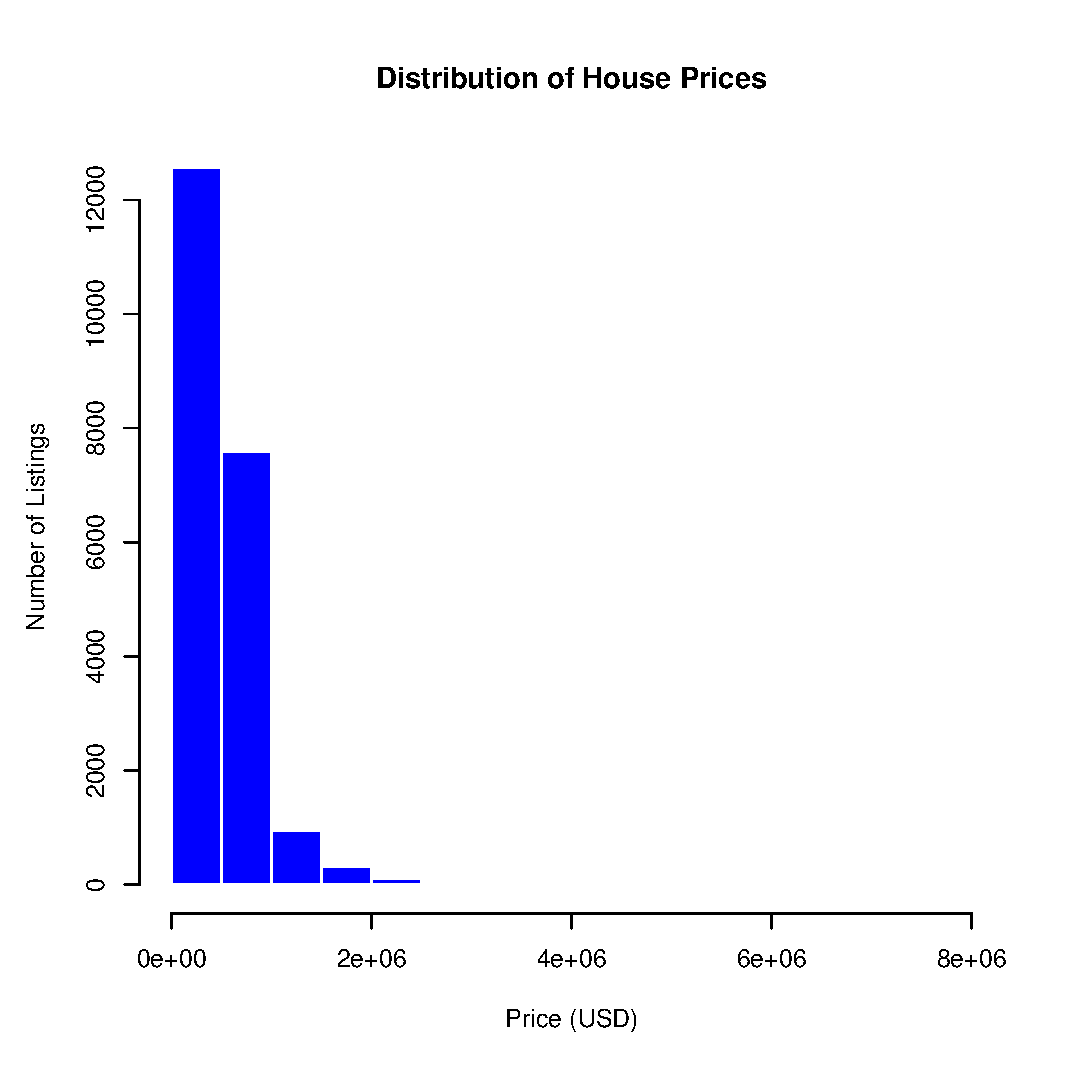
\includegraphics[width=0.75\textwidth,height=0.52\textwidth]{hist_housing_default.eps}
    \label{figure6} 
\end{figure}
(Data source: \href{https://raw.githubusercontent.com/rashida048/Datasets/master/home_data.csv}{House Data}, \textcolor{red}{breaks = "Sturges"})

\newpage
{\LARGE{\textbf{Histogram of house prices using Scott's Rule}}}
\vskip25pt

\begin{figure}[h]
\centering
      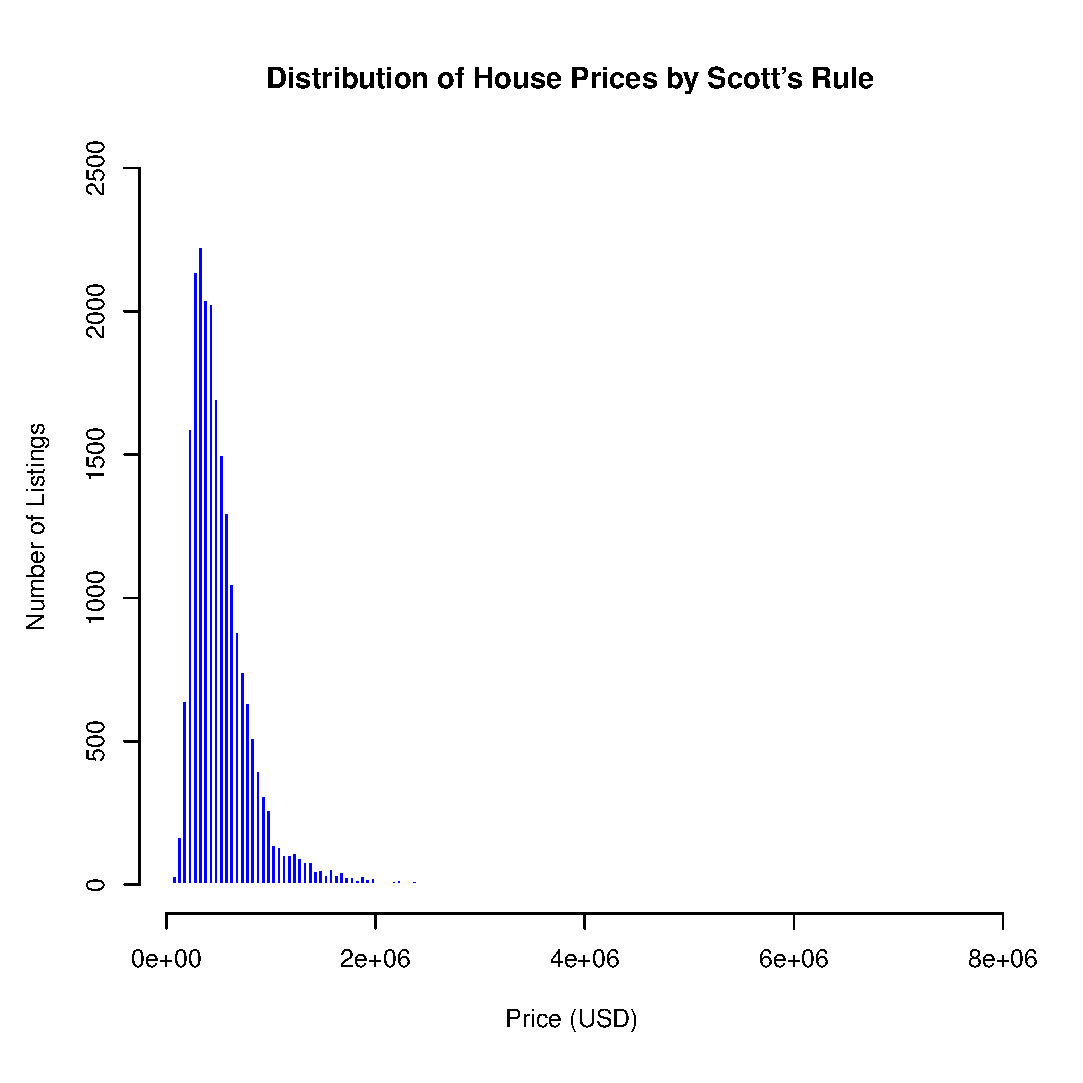
\includegraphics[width=0.75\textwidth,height=0.52\textwidth]{hist_housing_Scott.eps}
    \label{6} 
\end{figure}
(Data source: \href{https://raw.githubusercontent.com/rashida048/Datasets/master/home_data.csv}{House Data}, \textcolor{red}{breaks = "Scott"})

\newpage
{\LARGE{\textbf{Histogram of house prices using Freedman-Diaconis's Rule}}}
\vskip25pt

\begin{figure}[h]
\centering
      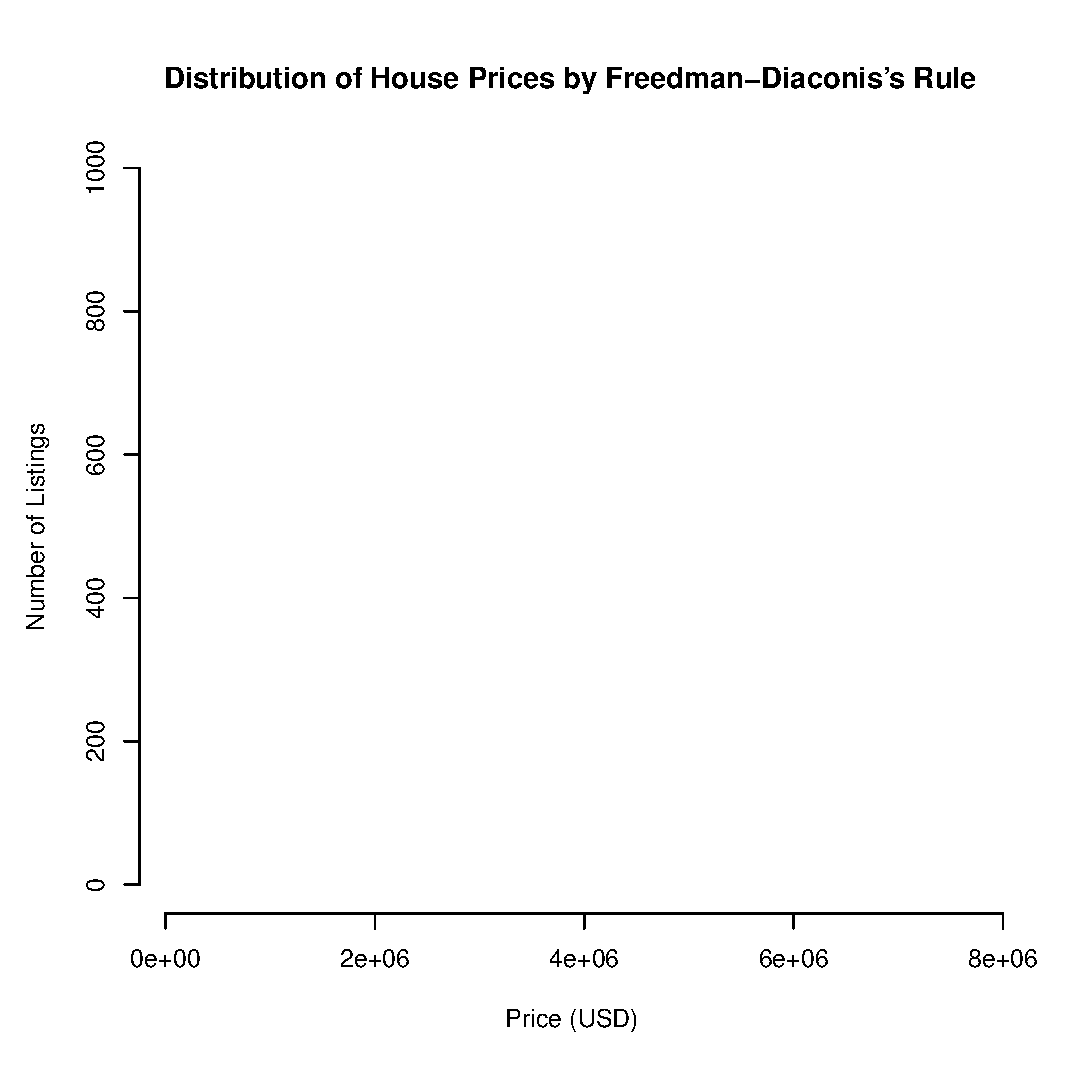
\includegraphics[width=0.75\textwidth,height=0.52\textwidth]{hist_housing_Freedman.eps}
    \label{figure7} 
\end{figure}
(Data source: \href{https://raw.githubusercontent.com/rashida048/Datasets/master/home_data.csv}{House Data}, \textcolor{red}{breaks = "Freedman-Diaconis"})

\newpage
{\LARGE\centerline{\textbf{Consistency}}}
\vskip25pt
\begin{minipage}{.9\textwidth}
    \Large 
\begin{defi}[\cite{garthwaite02}]
    An estimator $\hat{\theta}$ for $\theta$ is (weakly) consistent if $\IP(|\hat{\theta}-\theta|>\epsilon)\to0$ as $n\to\infty$ for any $epsilon>0$, i.e. $\hat{\theta}$ converges to $\theta$ in probability.
\end{defi} 
{\bf Claim:} ${\rm MSE}\{\hat{\theta}\}\to0$ implies consistency. 
\begin{eqnarray*}
    \IP(|\hat{\theta}-\theta|>\epsilon)=\E\left[\bone_{\{|\hat{\theta}-\theta|>\epsilon\}}\right]&\le&\E\left[\frac{|\hat{\theta}-\theta|^2}{\epsilon^2}\bone_{\{|\hat{\theta}-\theta|>\epsilon\}}\right]\\
    &\le&\epsilon^{-2}\E\left[|\hat{\theta}-\theta|^2\right].
\end{eqnarray*}
\end{minipage}

\newpage
{\LARGE\centerline{\textbf{Cumulants}}}
\vskip25pt
\begin{minipage}{.9\textwidth}
    \large 
  \begin{itemize}
    \item[$\blacktriangleright$] Moments and moment generating function (MGF)
    \begin{equation*}
        \E\left(e^{tX}\right)=\sum_{n\ge0}\frac{t^n}{n!}\E(X^n).
    \end{equation*}
    \item[$\blacktriangleright$] $\log$-MGF: Cumulants and their generating function
\begin{equation*}
    \log\E\left(e^{tX}\right)=\sum_{n\ge0}\frac{t^n}{n!}\kappa_n(X).
\end{equation*}
    \item[$\blacktriangleright$] Cumulants to moments:
\begin{eqnarray}
    \kappa_1(X)&=&\E(X),\nonumber\\
    \kappa_2(X)&=&\E[(X-\E[X])^2],\nonumber\\
    \kappa_3(X)&=&\E[(X-\E[X])^3],\nonumber\\
    \kappa_4(X)&=&\E[(X-\E[X])^4]-3(\E[(X-\E[X])^2])^2.\nonumber
\end{eqnarray}
    \item[$\blacktriangleright$] Skewness  $\kappa_3/\kappa_2^{3/2}$, and 
  \end{itemize}
\end{minipage}

\newpage
{\LARGE\centerline{\textbf{Landau's symbol}}}
\vskip25pt
\begin{minipage}{.9\textwidth}
   \Large
   We also recall the following standard notation for the asymptotic behavior of the relative order of magnitude of two functions $f(n)$ and $g(n )>0$ as $n$ tends to infinity.
   We write
   \begin{itemize}
      \item
        $f(n)=O(g(n))$,
        or $f(n ) \lesssim g(n )$, if $\limsup_{n \to\infty} f(n ) / g(n ) <\infty$;
      \item
        $f(n)=\Omega(g(n ))$, or 
        $f(n ) \gtrsim g(n )$, if $\liminf_{n \to\infty} f(n) / g(n)>0$;
    % \item       $f(\lambda )=\Theta(g(\lambda ))$ if $f(\lambda )=O(g(\lambda ))$ and $f(\lambda )=\Omega(g(\lambda ))$, 
      \item $f(n)\asymp g(n)$ if $f(n)=O(g(n))$ and $f(n)=\Omega(g(n))$; % if $f(\lambda )=\Theta(g(\lambda ))$;
  % \item $f(\lambda )\sim g(\lambda )$ if $\lim_{\lambda \to \infty} f(\lambda )/g(\lambda ) = 1$, 
     \item $f(n)=o(g(n))$, if $f(n)/g(n)\to 0$;
  %    \item $f(x)\ll g(x)$, or $g(x)\gg f(x)$ if $f(x)\ge0$ and $f(x)=o(g(x))$.
      \item $f(n)\ll g(n)$, or $g(n)\gg f(n)$, if $f(n)\ge0$ and $f(n)/g(n)\to 0$.
  \end{itemize}
  Find more details in this Wikipedia page of \href{https://en.wikipedia.org/wiki/Big_O_notation#History_(Bachmann–Landau,_Hardy,_and_Vinogradov_notations)}{Big O notation}.
\end{minipage}







\newpage
\bibliographystyle{apalike}
% \bibliography{../ref}
\begin{thebibliography}{}

    \bibitem[Boyd and Steele, 1978]{boydsteele78}
    Boyd, D.~W. and Steele, J.~M. (1978).
    \newblock Lower bounds for nonparametric density estimation rates.
    \newblock {\em Ann. Statist.}, 6(4):932--934.
    
    \bibitem[Doane, 1976]{doane76}
    Doane, D.~P. (1976).
    \newblock Aesthetic frequency classifications.
    \newblock {\em Amer. Statist.}, 30(4):181--183.
    
    \bibitem[Dudley, 2002]{Dudley02}
    Dudley, R.~M. (2002).
    \newblock {\em Real Analysis and Probability}.
    \newblock Cambridge Studies in Advanced Mathematics. Cambridge University Press, Cambridge, 2 edition.
    
    \bibitem[Freedman and Diaconis, 1981]{FreedmanDiaconis81}
    Freedman, D. and Diaconis, P. (1981).
    \newblock On the histogram as a density estimator: $L_2$ theory.
    \newblock {\em Probab. Theory Related Fields}, 57(4):453--476.
    
    \bibitem[Garthwaite et~al., 2002]{garthwaite02}
    Garthwaite, P.~H., Jolliffe, I.~T., and Jones, B. (2002).
    \newblock {\em Statistical inference}.
    \newblock OUP Oxford.
    
    \bibitem[Scott, 1979]{scott79}
    Scott, D.~W. (1979).
    \newblock {On optimal and data-based histograms}.
    \newblock {\em Biometrika}, 66(3):605--610.
    
    \bibitem[Scott, 2015]{scott15}
    Scott, D.~W. (2015).
    \newblock {\em Multivariate density estimation: theory, practice, and visualization}.
    \newblock Wiley Series in Probability and Statistics. John Wiley \& Sons, 2nd edition.
    
    \bibitem[Sturges, 1926]{sturges26}
    Sturges, H.~A. (1926).
    \newblock The choice of a class interval.
    \newblock {\em J. Amer. Statist. Assoc.}, 21(153):65--66.
    
    \end{thebibliography}
    
\end{document}